\documentclass[hidelinks, 12pt]{article}
\usepackage{fontspec}
\usepackage{xunicode}
\usepackage[french]{babel}

\usepackage{csquotes}
\usepackage[style=verbose-ibid,backend=bibtex]{biblatex}

\usepackage{hyperref}
\usepackage{enumitem}
\usepackage{setspace}
\usepackage{lscape}
\usepackage{graphicx}
\usepackage{float}

\usepackage{soul}
\usepackage{color}
\usepackage[dvipsnames]{xcolor}
\usepackage{listings}

\newcommand{\code}[1]{\colorbox{LightGray}{\texttt{#1}}}

\definecolor{LightGray}{rgb}{0.97,0.97,0.97}
\definecolor{red}{RGB}{255,0,0}
\definecolor{brown}{RGB}{139,69,19}
\definecolor{green}{RGB}{0,128,0}
\definecolor{blue}{RGB}{0,0,255}

\lstdefinelanguage{SPARQL}{
	basicstyle=\small\ttfamily,
	backgroundcolor=\color{LightGray},
	%	
	tabsize=1,
	showstringspaces=false,
	columns=fullflexible,
	breaklines=true,
	breakatwhitespace=true,
	%
	aboveskip=1em,
	belowskip=1em,
	xleftmargin=.5em,
	xrightmargin=.5em,
	framexleftmargin=.5em,
	framextopmargin=.5em,
	framexbottommargin=.5em,
	framexrightmargin=.5em,
	%
	morekeywords=[1]{paysLabel,population,date,cio,pays,populationStatement,noc,geopoint},
	keywordstyle=[1]\color{green},
	%
	morekeywords=[2]{wd,Q6256,wdt,P31,p,P1082,ps,pq,P585,wikibase,P984,label,bd,serviceParam,language,P625},
	keywordstyle=[2]\color{MidnightBlue},
	%
	morekeywords=[3]{SELECT,ORDER,BY,WHERE,FILTER,YEAR,NOW,SERVICE,DISTINCT},
	keywordstyle=[3]\color{red},
	%
	morestring=[b][\color{brown}]",
	otherkeywords={?},
}

\lstdefinelanguage{python}{
	basicstyle=\small\ttfamily,
	backgroundcolor=\color{LightGray},
	%	
	tabsize=1,
	showstringspaces=false,
	columns=fullflexible,
	breaklines=true,
	breakatwhitespace=true,
	%
	aboveskip=1em,
	belowskip=1em,
	xleftmargin=.5em,
	xrightmargin=.5em,
	framexleftmargin=.5em,
	framextopmargin=.5em,
	framexbottommargin=.5em,
	framexrightmargin=.5em,
	%
	morekeywords=[1]{import,as,for,in,True},
	keywordstyle=[1]\color{Fuchsia},
	%
	morekeywords=[2]{FMI\_prepared2,FMI\_prepared2\_df,colonnes\_a\_traiter,colonne,condition,keep,subset,FMI\_Python},
	keywordstyle=[2]\color{MidnightBlue},
	%
	morekeywords=[3]{dataiku,pandas,pd},
	keywordstyle=[3]\color{green},
	%
	morestring=[b][\color{brown}]",
	morestring=[b][\color{brown}]',
	otherkeywords={?},
}

\bibliography{Journal-de-bord-bibliographie}

\title{Projet Jeux Olympiques - Journal de bord}
\date{Janvier 2024}
\author{T. Burnel, N. Grim, M. Griveau, M. Mechentel}

\begin{document}

\setstretch{1.5}
\maketitle





%





\section{Introduction}

Nous somme une équipe de datajournalistes chargée, à l'approche des Jeux Olympiques de Paris, d'étudier l'existence ou non de liens entre le succès d'une pays aux Jeux et sa richesse. Notre hypothèse de départ est la suivante : les pays développés gagnent significativement plus de médailles en raison de leur niveau d'investissement dans le domaine sportif. 

À l'aune de l'examen et du traitement des données que nous avons à notre disposition, nous avons pour ambition de déterminer si la politique d'investissement dans les infrastructures sportives des pays a une quelconque influence sur leurs résultats aux épreuves des Jeux.

Notre travail sera divisé en deux temps. Nous mettrons en relief le nombre de médailles remportées par les pays lors de six éditions des Jeux Olympiques (1996, 2000, 2004, 2008, 2012, 2016) par rapport à leur population, leur Produit Intérieur Brut, au pourcentage de ce dernier investi dans le domaine sportif. Un second temps sera consacré à l'examen de la réussite de la France et du Royaume-Uni aux épreuves de natation sur la base du nombre d'infrastructures relatives pour 100.000 habitants.

Le choix de ces pays repose sur divers points de convergence : leur nombre d'habitants, leur économie et leur qualité de pays organisateur des Jeux. 

Le résultat du traitement des données constituera une base à la réalisation de datavisualisations et d'une application web exploitables pour l'écriture d'articles journalistiques sur le sujet des Jeux Olympiques.





%





\section{Jeux de données}

\subsection{Jeux du premier \textit{flow}}

Notre premier \textit{flow} concerne les médailles remportées par les pays lors des six éditions des Jeux Olympiques sur lesquelles nous avons décidé de travailler. En amont du traitement, nos jeux étaient au nombre de deux. Le premier présente le nombre de médailles remportées par sportif aux Jeux sur une période de 120 ans\autocite{kaggle}. Le deuxième, le Produit Intérieur Brut des pays et son pourcentage investi dans le domaine sportif\autocite{fmi}.

Nous avons enrichi ces jeux grâce au résultat d'une requête SPARQL, saisie sur le service de Wikidata. Le jeu ainsi produit présente le nombre d'habitants de l'ensemble des pays répertoriés dans la base de Wikidata, sur une période de trente ans (1993 - 2023)\autocite{wikiquerypop}.

Trois autres jeux ont dû faire leur entrée au cours du traitement pour pallier de nombreux manquements. Nous avons constaté qu'en dépit d'indiquer le pourcentage du Produit Intérieur Brut investi dans le domaine sportif, le jeu du Fonds Monétaire International ne contenait pas le PIB des pays. Nous avons introduit un jeu de la Banque mondiale\autocite{worldbank} dans le \textit{flow} -- lequel contient le montant du PIB avec une profondeur chronologique suffisante.

Les deux autres jeux concernent un problème de coordonnées. Lorsque Dataiku identifie des données de type \textit{country}, nous pensions pouvoir en récupérer les coordonnées -- notamment afin de les exploiter pour les datavisualisations. L'extension \textit{reverse geocoding plugin} aurait pu nous le permettre, sans succès. Nos suppositions portent sur notre version gratuite de Dataiku et de son nombre réduit de fonctionnalités.

Ne disposant d'aucun budget pour disposer d'une version payante, nous avons recherché un jeu contenant les coordonnées des pays et l'avons trouvé sur la plateforme GitHub\autocite{github}. Nonobstant, les longitudes et latitudes des pays ainsi récupérées se sont avérées être fautives le moment des datavisualisations venu. C'est pourquoi nous avons mis au point une deuxième SPARQL, capable de renvoyer les bonnes coordonnées de tous les pays présents dans la base de Wikidata. Le jeu ainsi récupéré correspond au dernier renfort dont nous avons eu besoin pour être en mesure de réaliser des datavisualisations.





%





\subsubsection{Jeu de Kaggle}

Le jeu est composé de 15 colonnes et 271.117 lignes. 7 colonnes fournissent des informations sur les athlètes (\textit{ID}, \textit{Name}, \textit{Sex}, \textit{Age}, \textit{Height}, \textit{Weight}, \textit{Medal}) ; 2 colonnes sur leurs pays (\textit{Team}, \textit{NOC}) et 6 sur les éditions des Jeux Olympiques (\textit{Games} ; \textit{Year} ; \textit{Season} ; \textit{City} ; \textit{Sport} ; \textit{Event}).

Les données sont exprimées en langue anglaise. La casse des chaînes de caractère suit le schéma d'une majuscule à chaque nouveau mot -- exception faite des unités de mesure dans la colonne \textit{Event} (comprendre \textit{Épreuve}) : le terme \textit{metres} est toujours noté en bas-de-casse. Les données sur la taille et le poids des athlètes sont des entiers. 2 colonnes, \textit{Games} et \textit{Year} contiennent des données de date, exprimées en année. La colonne \textit{Games} a ceci de particulier qu'elle agrège une donnée de date et une donnée textuelle. Les Jeux Olympiques d'été de 1992 sont notés \enquote{1992 Summer}.

Le jeu ne présente pas de défauts majeurs sur les colonnes que nous comptons conserver lors du traitement. Un problème plus préoccupant concerne la dénomination des pays, parfois obsolète (\textit{Soviet Union}, \textit{West Germany}) ou impropres (\textit{Japan-1}, \textit{Switzerland-2}). Nous effectuerons les jointures sur le code NOC des pays (un code unique attribué par le \textit{National Olympic Committee} -- le Comité National Olympique) pour plus de fiabilité.





%





\subsubsection{Jeu du FMI}

Le jeu est composé de 42 colonnes pour 7.715 lignes. La colonne \textit{Country Name} permet d'identifier les pays. Celle nommée \textit{COFOG Function Name} correspond au secteur des investissements et a pour unique valeur \textit{Expenditure on recreational \& sporting services}. La colonne \textit{Unit Name} précise l'échelle de calcul des investissements (soit en pourcentage du PIB, \textit{Percent of GDP}, soit en monnaie courante \textit{Domestic currency}). Le montant des investissements est renseigné sur 30 colonnes (1993 - 2022).

Les 9 autres colonnes correspondent à des codes et des dénominations propres au FMI (\textit{Country Code}, \textit{COFOG Function Code}, \textit{Sector Name}, \textit{Sector Code}, \textit{Unit Code}, \textit{Attribute}, \textit{Indicator Code}, \textit{Global DSD Time Series Code}, \textit{col\_41}). Le potentiel de croisement avec d'autres jeux étant par la force des choses très limité, nous n'utiliserons pas ces données.  

L'ensemble du jeu est rédigé en langue anglaise. Noms de pays, sigles, codes, acronymes et unités de mesure (notées \enquote{Cash}, \enquote{Non Cash}, \enquote{Gross}, \enquote{Net}) à part, la casse des données textuelles implique la présence d'une seule majuscule en début de chaîne. Nous notons l'utilisation de caractères spéciaux, à l'instar de l'esperluette ou de la barre oblique.

Exception faite des \textit{Country Code} et du code correspondant à la valeur \enquote{Domestic currency}, l'intégralité des codes sont un mélange de caractères numériques et textuels en haut-de-casse (\enquote{S13112} pour la colonne \textit{Sector Code} ou \enquote{XDC\_R\_B1GQ} dans la colonne \textit{Unit Code}).

Les noms de pays souffrent d'un problème d'harmonisation et d'actualité (\textit{West Bank and Gaza}, \textit{Russian Federation}, \textit{China, P.R.: Mainland}).

Ce jeu est de loin le moins bien structuré et le plus fautif. Bien que nous ne comptions pas les conserver au cours du traitement, les trois dernières colonnes (\textit{Indicator Code}, \textit{Global DSD Time Series Code}, \textit{col\_41}) sont d'une opacité confondante et témoignent du problème majeur du jeu : énormément de données sont vides, nulles ou incompréhensibles (\enquote{GERS\_G14\_GDP\_PT} pour la colonne) \textit{Indicator Code}, \enquote{A|GB|S1311|W0|S1|G2M|\_Z|\_Z|GF0801|
	XDC|\_T|\_X} pour la colonne \textit{Global DSD Time Series Code}).
également
Au sein des colonnes correspondant au montant des investissements par année, se côtoient des lignes vides et des sigles (\enquote{NA}, \enquote{NP}, \enquote{AC}), sans justification ni harmonisation aucune. En somme, ce jeu représente un véritable enjeu de nettoyage et de croisement des données.





%





\subsubsection{Jeu de Wikidata (population)}

En préambule de l'analyse du jeu de Wikidata, revenons un instant sur l'élaboration de la requête nous ayant permis de l'obtenir. Celle-ci renvoie le nombre d'habitants de l'ensemble des pays présents dans la base de données de Wikidata, sur une période de trente ans (1993 - 2023) :

\label{query1}\begin{lstlisting}[language=SPARQL]
SELECT ?paysLabel ?population ?date ?cio
WHERE 
{
	?pays wdt:P31 wd:Q6256.
	?pays wdt:P984 ?cio.
	?pays p:P1082 ?populationStatement.
	?populationStatement ps:P1082 ?population. 
	?populationStatement pq:P585 ?date.
	FILTER(YEAR(?date) >= (YEAR(NOW()) - 30)).
	SERVICE wikibase:label { bd:serviceParam wikibase:language "[AUTO_LANGUAGE],fr". }
}
ORDER BY ?paysLabel ?date
\end{lstlisting}

Être en mesure de requêter l'intégralité des pays a été la première étape de la construction de notre requête. Le premier triplet permet de spécifier la nature -- notée \code{wdt:P31} -- de notre variable inconnue \code{?pays} en la faisant correspondre à l'objet \code{country} -- noté \code{wd:Q6256} :

\begin{lstlisting}[language=SPARQL]
	?pays wdt:P31 wd:Q6256.
\end{lstlisting}

Le deuxième triplet constitue un ajout tardif, destiné à faciliter les jointures avec les autres jeux de données. Comme nous travaillons sur les Jeux Olympiques, les pays peuvent être non seulement identifiés par les codes basés sur la norme ISO 3166 mais aussi par les codes du CIO (Comité International Olympique). Nous avons donc récupéré cette donnée grâce à la propriété Wikidata correspondante -- notée \code{wdt:P984} :

\begin{lstlisting}[language=SPARQL]
	?pays wdt:P984 ?cio.
\end{lstlisting}

La deuxième partie de notre requête doit renvoyer le nombre d'habitants par pays en prenant en compte une dimension chronologique. La complexité de cette demande requiert un parcours de graphique en quatre temps.

Pour ce faire, nous avons consulté la liste de préfixes\autocite{wikiprefixes} de Wikidata afin de créer une nouvelle variable, \code{?populationStatement}. Le troisième triplet a recours à la classe \code{population} -- notée \code{p:P1082} -- et signifie que la variable \code{?populationStatement} a pour valeur la population des pays :

\begin{lstlisting}[language=SPARQL]
	?pays p:P1082 ?populationStatement.
\end{lstlisting}

L'obtention du nombre d'habitants a nécessité le recours au préfixe \code{ps}, lequel permet de récupérer la valeur de la propriété relative à la population :

\begin{lstlisting}[language=SPARQL]
	?populationStatement ps:P1082 ?population.
\end{lstlisting}

Enfin, nous avons rédigé le dernier triplet sur la base du préfixe \code{pq} pour attribuer la valeur chronologique à la variable \code{?date}. Un filtre y a été appliqué pour exprimer les limites extrêmes de notre période, soit \code{NOW} pour 2023 et \code{-30} pour 1993 :

\begin{lstlisting}[language=SPARQL]
	?populationStatement pq:P585 ?date.
	FILTER(YEAR(?date) >= (YEAR(NOW()) - 30)).
\end{lstlisting}

La première et dernière ligne permettent de cadrer l'affichage des résultats. Lorsque la requête s'exécute, Wikidata renvoie le nom de chaque pays (\code{?paysLabel}) par ordre alphabétique, le nombre d'habitants (\code{?population}) et l'année correspondante (\code{?date}) par ordre croissant :

\begin{lstlisting}[language=SPARQL]
	SELECT ?paysLabel ?population ?date
	ORDER BY ?paysLabel ?date
\end{lstlisting}

Nous nous sommes heurtés à plusieurs obstacles avant de rendre la requête fonctionnelle. Il nous a fallu un certain temps avant de comprendre la nécessité d'un parcours de graphique en quatre temps et du recours à une variable telle que \code{?paysStatement}. À cet égard, la documentation sur l'utilisation des propriétés \code{population}\autocite{wikipop} et \code{date}\autocite{wikidate} a été d'un grand secours. 

Nous avons également pris en exemple la requête \emph{Population in Europe after 1960}\autocite{wiki1960}. La consulter a été l'occasion d'une meilleure compréhension des propriétés Wikidata ainsi qu'une porte ouverte à la lecture de la documentation et à l'appréhension des requêtes en deux temps (collecte des propriétés d'une classe puis requêtage en fonction de notre besoin).

La rédaction de cette première requête a été d'une grande aide pour les autres recours à Wikidata qui ont émaillé notre chaîne de traitement.
\newline

Le jeu ainsi généré est composé de 13 colonnes et 3.737 lignes. Les lignes de la colonne, \textit{paysLabel.xml:lang} sont composées d'une même et unique donnée : \enquote{fr}. Il s'agit de langue dans laquelle les noms des pays sont renvoyés. 

\label{query1tab}Sur les 12 colonnes restantes, 6 fonctionnent selon une logique de duo et 6 autres selon une logique de trio. Pour chaque donnée, le jeu indique sont \textit{type}, sa \textit{value} et, pour les trio, son \textit{datatype}. Ainsi, la donnée \enquote{cio} fait l'objet de 2 colonnes : \textit{cio.type}, \textit{cio.value} (\textit{idem} pour les données \enquote{isoCode} et \enquote{paysLabel}) et la donnée \enquote{date} fait l'objet de 3 colonnes : \textit{date.datatype}, \textit{date.type}, \textit{date.value} (\textit{idem} pour la donnée \enquote{population}). 

Bien que notre requête ne précise vouloir recueillir ni le \textit{type} ni le \textit{datatype} des données, ces colonnes sont malgré tout présentes dans le jeu de sortie. Les données textuelles sont exprimées en anglais (mis à part les noms de pays) et sont en bas-de-casse -- exception faite des sigles et des noms de pays. Les dates sont exprimées selon le schéma YYYY-MM-DDThh\!\!:mm\!\!:ssZ. L'intégralité des \textit{types} correspondent à \enquote{literal}. Les colonnes \textit{datatype} ont pour valeur des liens renvoyant à des schémas XML du W3C.

Le jeu est d'une propreté exemplaire, les données sont harmonisées et correctement typées, ce qui nous sera d'une grande aide lors des jointures.





%





\subsubsection{Jeu de la Banque mondiale}

Le jeu se compose de 68 colonnes pour 533 lignes. Chaque ligne pleine est en réalité séparée de la suivante par une ligne vide. De surcroît, la dernière colonne est intégralement vide et ne porte que le sommaire nom de \textit{col\_67}. Sur l'ensemble du jeu, 63 colonnes correspondent aux années pour lesquelles le PIB des pays est renseigné (1960- 2022). 2 autres colonnes donnent des informations sur les pays : leur nom, leur code (\textit{Country Name}, \textit{Country Code}) et les 2 restantes, sur la donnée économique -- en l'occurrence le PIB (\textit{Indicator Name}, \textit{Indicator Code}), en dollars courant. 

Les données textuelles sont en langue anglaise. Les noms des pays portent une majuscule initiale. Les codes sont exclusivement en haut-de-casse. Les données numériques sont exprimées en décimaux.

Notons que certaines entrées de la colonne \textit{Country Name} témoignent d'une certaine originalité dans la mesure où ils ne sont pas références à des pays nommément explicites (\enquote{Heavily indebted poor countries (HIPC)}, \enquote{IBRD only}, \enquote{Low \& middle income}, etc.). Ces excentricités soulignent l'importance des codes des pays pour effectuer les jointures et faire l'économie des entrées impropres. Enfin, les premières décennies souffrent d'un cruel manque de données mais plus nous avançons dans le temps, plus le jeu est complet sur l'ensemble des pays.





%





\subsubsection{Jeu de GitHub}

Le jeu se compose de 6 colonnes et 263 lignes. 2 de ces colonnes correspondent à la latitude et longitude (\textit{Latitude (average)}, \textit{Longitude (average)}) des pays dont le nom nous est donné dans la colonne \textit{Country}. Les trois autres colonnes (\textit{Alpha-2 code}, \textit{Alpha-3 code}, \textit{Numeric code}) correspondent à des codes de pays prévus par la norme ISO 3166-1.

Les données textuelles sont exprimées en langue anglaise. Nonobstant, nous comptons nous appuyer sur les codes des pays pour réaliser les jonctions. Le jeu ne présente aucune donnée manquante. 





%





\subsubsection{Jeu de Wikidata (coordonnées)}

Revenons derechef sur le détail de notre requête SPARQL, rédigée pour nous permettre de récupérer les coordonnée des pays recensés dans la base de données de Wikidata :

\begin{lstlisting}[language=SPARQL]
SELECT DISTINCT ?paysLabel ?geopoint ?noc
WHERE 
{
	?pays wdt:P31 wd:Q6256.
	?pays wdt:P984 ?noc.
	?pays wdt:P625 ?geopoint
	SERVICE wikibase:label { bd:serviceParam wikibase:language "[AUTO_LANGUAGE],en". }
}
\end{lstlisting}

Nous indiquons vouloir récupérer les données selon les colonnes suivantes : le nom du pays (noté \code{?paysLabel}), leurs coordonnées (notées \code{?geopoint}) et leur code CIO (noté \code{?noc}) :

\begin{lstlisting}[language=SPARQL]
	SELECT DISTINCT ?paysLabel ?geopoint ?noc
\end{lstlisting}

Le premier triplet est \textit{stricto sensu} le même que celui de notre première requête Wikidata sur les populations (\textit{cf}. \textit{supra} p. \pageref{query1}).

Il permet de signifier que notre variable inconnue \code{?pays} est de nature (notée \code{wdt:P31}) \enquote{pays} (noté \code{wd:Q6256}) :

\begin{lstlisting}[language=SPARQL]
	?pays wdt:P31 wd:Q6256.
\end{lstlisting}

Le deuxième triplet est également tout à fait similaire à son homonyme de la requête sur les populations (\textit{cf}. \textit{supra} p. \pageref{query1}). Il assigne à la variable \code{?noc} les codes des pays prévus par le Comité Olympique International grâce à la propriété relative notée \code{wdt:P984} :

\begin{lstlisting}[language=SPARQL]
	?pays wdt:P984 ?noc.
\end{lstlisting}

Enfin, le dernier triplet récupère les coordonnées géographiques des pays grâce à la propriété correspondante, notée \code{wdt:P625} :

\begin{lstlisting}[language=SPARQL]
	?pays wdt:P625 ?geopoint
\end{lstlisting}

Il en ressort un jeu composé de 8 colonnes et 185 lignes. Il présente la même logique de duo et de trio que notre autre jeu Wikidata (\textit{cf}. \textit{supra} p. \pageref{query1tab}) : les données \enquote{noc} et \enquote{paysLabel} font l'objet de 2 colonnes et les coordonnées, \enquote{geopoint}, font l'objet de trois colonnes. La longitude et la latitude sont regroupées au sein de la même colonne, \textit{geopoint.value} et sont présentées comme suit : \enquote{Point(<longitude> <latitude>)}. L'Islande a ainsi pour coordonnées \enquote{Point(-19.0 65.0)}.

Cette requête ayant été saisie dans l'urgence de devoir déboguer la réalisation des datavisualisations et la rédaction du présent journal de bord à moins d'une semaine de la date butoir, les noms de pays sont exprimés en langue anglaise et les résultats n'ont pas été ordonnés par ordre alphabétique à l'instar de la requête sur la population. Nonobstant, la forme des données qui nous préoccupent -- en l'occurrence, les codes NOC et les coordonnées -- ne dépend pas de la langue pourvu que l'alphabet soit le même.





%





\subsection{Jeux du second \emph{flow}}

Notre deuxième \emph{flow} repose sur la comparaison entre les investissements de la France et du Royaume-Uni, en l'occurrence à l'endroit des infrastructures de natation. En amont du traitement, nos jeux de données étaient au nombre de trois et présentent les informations suivantes :

\begin{itemize}
	\item Investissements dans les infrastructures sportives en France\autocite{ministere} ;
	\item Investissements dans les infrastructures sportives au Royaume-Uni\autocite{ru}.
\end{itemize}


\subsubsection{Jeu du ministère des sports et des jeux olympiques et paralympiques}

Le jeu présente 114 colonnes pour 143192 lignes. Par souci de concision, nous ne nous attarderons que sur les données qui seront conservées. Les colonnes concernées sont \emph{Type d'équipement sportif} et \emph{Commune Ancienne}, laquelle renseigne les codes postaux.

Sur l'ensemble du jeu, les données sont grossièrement saisies. Les \emph{Type d'équipement sportif} sont par exemple au nombre de 354 sans harmonisation commune dans la nomenclature avec présence de données aberrantes (citons \enquote{3 2}, \enquote{PETIT MORNAS} ou encore \enquote{Puy}). Nous nous appuierons sur la colonne \emph{Commune Ancienne} non pas sur la colonne \emph{Région Nom} car les données sont également mal saisies et aberrantes (\enquote{CC du Pays Châtillonnais}, \enquote{4.84405}, etc.).

\subsubsection{Jeu de Sport England}

À l'endroit du Royaume-Uni : deux jeux nous intéressent. Le premier, nommé \emph{Geographics} présente -- sur 25 colonnes et 118655 lignes -- des données géographiques à propos d'infrastructures sportives. Chaque infrastructure possède son ID (\emph{FacilityID}) et est rattachée à une région. Les autres colonnes fournissent des informations à propos des régions, selon un principe de colonne jumelles avec d'une part les ID, d'autre part les noms (Parliamentary Constituency ID ; Ward, Local Authority, Country, Active Partnership, Region). Deux colonnes concernent les coordonnées (\emph{Latitude} ; \emph{Longitude}).

Sur la propreté des données, certaines colonnes sont entièrement vides (\emph{Metro Name} ; \emph{Core City Name} ; \emph{LDP Code} ; \emph{LDP Name}) mais nous ne comptons pas les conserver au cours du traitement. Nonobstant, les données des coordonnées correspondent aux infrastructures, non pas aux régions. Cela pourra avoir des conséquences sur les visualisations dans la mesure où la myriade de points ne saura faire ressortir les contours des régions. 

Le second jeu se nomme \emph{SwimmingPool} et fournit des données sur la répartition des équipements de natation au Royaume-Uni. L'essentiel des colonnes donne des détails techniques sur les infrastructures (\emph{Length} ; \emph{Maximum Depth} ; \emph{Movable Floor} ; \emph{Seating}, etc.).

L'intégralité des données sont des entiers. Les entrées vides ou équivalentes à zéro sont derechef légion. Cependant, seule la colonne \emph{FacilityID} nous est nécessaire afin de réaliser des jointures avec le jeu \emph{Geographics}. 




















\section{Traitement des données}

\subsection{Objectif du traitement}

À l'aune de notre approche, notre premier \emph{flow} aura pour ambition de faire ressortir les données suivantes : les codes des pays attribués par le \emph{National Olympic Committee} -- que nous nous permettrons d'abréger \enquote{code NOC} -- le nombre de médailles remportées aux éditions six des Jeux Olympiques et le pourcentage d'investissement des pays dans le domaine sportif par rapport à leur PIB et à leur population.


\subsection{Chaîne de traitement du premier \emph{flow}}

\subsubsection{Préparation du jeu de la Banque Mondiale}

La première recette appliquée au jeu est une préparation. Elle consiste en la suppression de toutes les lignes vides -- soit une ligne sur deux, rappelons-le -- et en la conservation de seulement 7 colonnes sur 67 :
\begin{itemize}
	\item \emph{Country Code} ;
	\item Les éditions des Jeux de 1996 à 2016.
\end{itemize}
Les codes NOC seront fondamentaux pour réaliser de futures jointures et les années 1996, 2000, 2004, 2008, 2012 et 2016 correspondent aux limites chronologiques de notre approche.

Deux autres étapes composent la recette : le renommage des 7 colonnes restantes (ainsi, \emph{Country Code } et renommée \emph{NOC} et les colonnes des années sont renommées selon le même motif : \emph{1996} devient \emph{1996 - GDP} pour \emph{Gross Domestic Product}, c'est-à-dire le Produit Intérieur Brut.) et le passage de toutes les valeurs décimales en entiers, selon une logique d'arrondissement. 

\subsubsection{Préparation du jeu de Kaggle}

Ce jeu a fait l'objet de trois recettes. La première, une préparation, nous a permis de conserver uniquement 3 colonnes sur 15 :
\begin{itemize}
	\item \emph{NOC} ;
	\item \emph{Medal} ;
	\item \emph{Year}.
\end{itemize}
Nous avons également épuré la colonne \emph{Year} pour ne conserver que les années des Jeux relatives à notre sujet. Les entrées de la colonnes \emph{Medal} correspondant à des valeurs nulles (exemplairement \emph{N/A}) ont été supprimées. 

L'étape suivante consiste en la réalisation d'un pivot : les années présentes dans les lignes sont devenues des colonnes dont les lignes ont pris pour valeur les entrées de la colonne \emph{Medal}. 6 nouvelles colonnes ont donc été créées, une par édition des Jeux Olympiques, entre 1996 et 2016.

Enfin, nous avons compté les occurrences des trois types de médailles (bronze, argent, or) et créé des colonnes de sorties pour chaque type pour chaque édition. Par exemple, la colonne \emph{1996} a donné lieu à la création des colonnes \emph{1996 - Bronze} ; \emph{1996 - Silver} ; \emph{1996 - Gold}.

La deuxième recette est un \emph{group}. Le \emph{dataset} présente les médailles reportées par les athlètes, or nous n'avons conservé aucun donnée à leur endroit. Nonobstant, la répartition des médailles reposait toujours sur cette logique.

Nous avons donc réalisé un groupement pour réunir les doublons et compter les occurrences de chaque type de médaille remportée pour les six éditions des Jeux. Admettons qu'aux Jeux de 2016, un athlète français ait remporté une médaille de bronze et un autre deux. La recette a pour effet d'afficher le chiffre 3 pour l'entrée \enquote{France} sur la colonne \emph{2016 - Bronze}.

La troisième et dernière recette en amont des jointures est également une préparation. Elle nous a permis, pour chacune des six éditions, de créer une nouvelle colonne présentant la somme de toutes les médailles remportées par les pays. En guise d'exemple, nous savons qu'à l'édition de 2008, l'Australie a remporté un total de 110 médailles.

\subsubsection{Préparation du jeu de Wikidata}

L'enrichissement \emph{via} les données de Wikidata a été soumis a deux recettes. Une préparation où nous avons supprimé 8 colonnes -- lesquelles représentaient un considérable bruit documentaire dans la mesure où notre requête SPARQL ne les sollicitaient pas (exemplairement à propos des \enquote{types} de données : \emph{population.type}, \emph{date.type}, \emph{date.datatype}). 

Trois colonnes ont été renommées : \emph{cio.value} est devenu \emph{NOC} ; \emph{isoCode.value} est devenu \emph{Pays} et \emph{paysLabel.value} est devenu \emph{Nom - Pays}.

Nous avons modifié le format des dates : sur l'année, le jour, le mois et l'heure, nous n'avons conservé que l'année dans une colonne de sortie avant de supprimer la colonne initiale. Les années des six éditions mises à part, toutes les autres ont été supprimées et un nouveau pivot a été réalisé : les années en ligne sont passées en colonne et ont pris pour valeur le nombre d'habitants par pays. Ce pivot a permis la suppression des colonnes \emph{Année} et \emph{population.value}. Enfin, les colonnes des années ont été renommées selon un motif commun : \emph{1996} est devenu \emph{1996 - Pop}.

La dernière étape de cette recette consiste en la suppression de trois valeurs vides présentes dans la colonne \emph{NOC}.

À l'instar du jeu de Kaggle, nous avons appliqué une recette \emph{group} au jeu de Wikidata. Le groupe s'est effectué sur les colonnes \emph{NOC}, \emph{Pays} et \emph{Nom - Pays} afin de regrouper le nombre d'habitants par année sur une même ligne.

\subsubsection{Préparation du jeu de GitHub}

Le jeu de GitHub n'a nécessité qu'une maigre recette de préparation : nous avons supprimé les colonnes \emph{Alpha-2 Code} et \emph{Numeric Code} pour ne conserver que la colonne \emph{Alpha-3 Code} pour faciliter les jointures.

Nous avons également supprimé les entrées que Dataiku ne reconnaissait pas comme pays pour enfin renommer deux colonnes : \emph{Country} est devenu \emph{Pays} et \emph{Alpha-3 Code} est devenu \emph{Code}.

\subsubsection{Préparation du jeu du FMI}

À la faveur de la première recette, une préparation, nous avons supprimé de la colonne \emph{Unit Name} les lignes où la valeur était \emph{Domestic currency} pour ne conserver que le pourcentage du Produit Intérieur Brut (\emph{Percent of GDP}) investi par les pays dans le domaine du sport.

Nous avons uniquement conservé 7 colonnes : \emph{Country Name} ainsi que les dates des six éditions des Jeux. La dernière étape de la préparation consistait en la suppression de lignes vides pour la colonne \emph{2016}. À partir de cette étape, Dataiku se figeait et nous laissait dans l'impossibilité d'ajouter de nouvelles étapes. Nous avons donc dû ajouter une autre recette de préparation pour que le \emph{run} fonctionne et reprendre le traitement.

Dans cette deuxième préparation, les 6 colonnes correspondant aux éditions des Jeux selon le motif suivant : \emph{1996} devient \emph{1996 - FMI}. 

Il nous a fallu manuellement modifier 13 valeurs dans la colonne \emph{Country Name} pour une meilleure reconnaissance des pays par Dataiku. Par exemple : \emph{Russian Federation}, \emph{Czech Rep.} ne sont pas reconnus, tandis que \emph{Russia} et \emph{Czech Republic} le sont. Ces modifications ont donné lieu à la création d'une colonne de sortie \emph{Pays} car il nous était impossible de modifier les noms des pays directement dans la colonne d'origine. Nous avons naturellement supprimé la colonne \emph{Country Name}, une fois ces modifications effectuées. 

Nous avons rencontré un problème de valeurs aberrantes dans les valeurs indiquées pour les investissements par rapport au PIB. La nature du problème repose sur des conversions mathématiques fautives : les pour mille et pour cent ont subi la même opération. Nous avons donc entrepris de corriger ces données par l'intermédiaire d'une recette Python que voici :

\begin{lstlisting}[language=python]
import dataiku
import pandas as pd
from dataiku import pandasutils as pdu

FMI_prepared2 = dataiku.Dataset("FMI_prepared2")
FMI_prepared2_df = FMI_prepared2.get_dataframe()

colonnes_a_traiter = ['1996 - FMI', '2000 - FMI', '2004 - FMI', '2008 - FMI', '2012 - FMI', '2016 - FMI']

for colonne in colonnes_a_traiter:
				condition = FMI_prepared2_df[colonne] > 0.1
				FMI_prepared2_df.loc[condition, colonne] /= 10

FMI_prepared2_df.drop_duplicates(subset=['Pays'], keep='first', inplace=True)

FMI_Python = dataiku.Dataset("FMI_Python")
FMI_Python.write_with_schema(FMI_prepared2_df)
\end{lstlisting}

Le code ci-dessus intervient sur les colonnes des six éditions des Jeux :

\begin{lstlisting}[language=python]	
colonnes_a_traiter = ['1996 - FMI', '2000 - FMI', '2004 - FMI', '2008 - FMI', '2012 - FMI', '2016 - FMI']
\end{lstlisting}

Et modifie leur contenu grâce à une boucle \code{for} : si les colonnes contiennent des valeurs supérieures à \code{0.1}, ces dernières sont divisées par \code{10} pour obtenir la juste valeur d'investissement :

\begin{lstlisting}[language=python]
for colonne in colonnes_a_traiter:
				condition = FMI_prepared2_df[colonne] > 0.1
				FMI_prepared2_df.loc[condition, colonne] /= 10
\end{lstlisting}

La bonne valeur des données est ainsi rétablie, et l'ensemble de nos jeux sont prêts pour les jointures.

\subsubsection{Première jointure}

La première jointure concerne les jeux préparés de Kaggle et de Wikidata, sur la colonne \emph{NOC}. Il en résulte la création du jeu \emph{Med-Pop}, pour \enquote{Médailles-Population}. La jointure s'est réalisée sans suppression et n'a pas occasionné une perte significative d'informations.

\subsubsection{Deuxième jointure}

La deuxième jointure regroupe les jeux \emph{Med-Pop} et \emph{GDP} (jeu de la Banque mondiale) -- également sur la colonne \emph{NOC}, sans suppression ni perte significative d'informations. Le jeu \emph{Med-Pop-GDP} a ainsi été créé.

\subsubsection{Troisième jointure}

La troisième jointure est un croisement du jeu \emph{lien\_pays} (issu de GitHub) et du jeu \emph{FMI}, sur la colonne \emph{Pays} du jeu du FMI. Tous les pays reconnus dans le ce jeu-ci ont été enrichis par les données du jeu de GitHub, soit par les données de longitude, de latitude et par un code similaire au code NOC. Le jeu \emph{FMI-Liens} a ainsi été créé.

\subsubsection{Quatrième jointure}

Enfin, la quatrième jointure rassemble les jeux \emph{Med-Pop-GDP} et \emph{FMI-Liens} sur les colonnes \emph{Pays} (du jeu \emph{Med-Pop-GDP}) et \emph{Code} (du jeu \emph{FMI-Liens}). Dans la mesure où les médailles remportées constituent les données les plus importantes, la jointure a été réalisée de telle sorte à ce que les pertes touchent le jeu \emph{FMI-Liens} et non pas \emph{Med-Pop-GDP}.

\subsubsection{Préparation du jeu final}

Notre dernier jeu alors créé, \emph{Reunion}, a subi une recette de préparation afin de nettoyer les données une dernière fois. Les données sur la population ont été arrondies, les colonnes dont l'entête est en français ont été renommées pour harmoniser la nomenclature de notre \emph{dataset} de sortie. Enfin, les colonnes ont été organisées de la manière suivante : les deux premières colonnes sont \emph{NOC} et \emph{Country - Name} puis chaque édition des Jeux est présentée comme suit :

\begin{center}
	\begin{figure}[H]
		
\includegraphics[scale=0.4]{tableaufinal.png}
	\end{figure}
\end{center}


Et les deux dernières colonnes, \emph{Latitde (average)} et \emph{Longitude (average)} présentent les coordonnées géographiques des pays.


\subsection{Chaîne de traitement du second \emph{flow}}

SPARQL England :

Suppression de toutes les colonnes sauf 3 : geopoint.value ; RegionLabel.value ; population.value car c'est aussi du bruit documentaire.

Modification des valeurs de geopoint.value : from Point(0.41 52.24) 0.41 52.24.

Conservation d'une seule valeur de population par région + groupement pour avoir une seule ligne par région.

Renommage de certains noms de région pour faciliter la jointure


SWIMMINGPOOLS : conservation de la seule colonne \emph{FacilityID} pour faire la jointure partant du principe que 1 ID = 1 installation

GEOGRAPHICS : conservation de FacilityID, de Region Name et de Latitude et Longitude

1re jointure : SWIMMINGPOOLS et GEOGRAPHICS. Une inner join propre sur les ID, aucun souci. Donne le jeu \emph{InfraEnglandeJoin1}

2e jointure : SPARQL et InfraEnglandeJoin1. Jointure sur le nom de la région

Autre recette : group sur population.value avec copie de la colonne population pour la conserver.

Ensuite : produit en croix pour aboutir au nombre de piscine pour 100.000 habitants avec arrondissement pour cette colonne





POUR LA FRANCE

SPARQL, même opération. SPARQL a extrait toutes les régions de France mais nous n'avons gardé que celles de la France métropolitaine 

Jeu de la France : conservation des colonnes qui nous intéressent (type\_equipement, longitude, latitude, regionLabel, dans type équipement : remplacement de toutes les données qui nous intéressent en \enquote{piscine centre aquatique}

JOINTURE : inner join sur le nom de la region et le labelRegion 

JOINTURE : inner join aussi sur le nom de la région


Regroupement : jointure sur type\_equipement sans garder la longitude et la latitude 











\subsubsection{Semaine du 22 janvier 2024}

Mauvaise surprise : alors que nous voulions produire un autre flow afin de remplir la seconde partie de notre objectif et produire des datavisualisations comparant la France et le Royaume-Uni, un bogue manifestement causé par une installation relative à Javascript perturbe l'affichage sur Dataiku. Probablement : problèmes de compatibilité.

\begin{center}
	\begin{figure}[H]
		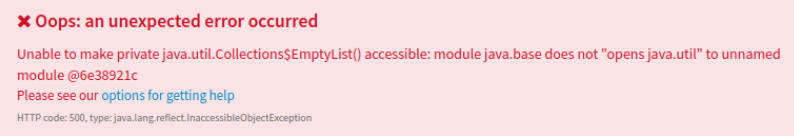
\includegraphics[scale=0.5]{bogue.png}
	\end{figure}
\end{center}

ll est probable que cette erreur soit apparue après l’installation d’une version de JDK supérieure à celle prise en charge par Dataiku. Il aurait ainsi fallu rétrograder notre version de JDK, mais nous craignons que cette manipulation entraîne des difficultés dans d’autres projets que nous menons. Nous ne pouvons dès lors nous appuyer que sur un seul ordinateur, qui possède une version inférieure de JDK, ce qui a causé d’importants soucis organisationnels à la fin du mois de janvier.

\subsection{Chaîne de traitement du second \emph{flow}}


\section{Visualisation des données}

\subsection{Présentation des visualisations}

\subsection{Analyse}

Qu'apprend-on en regardant les visualisations ? Quels sont les biais ?
\newpage


\section{Sitographie}
\printbibliography[heading=none]
\newpage

\tableofcontents

\end{document}